\section{User Story}

\begin{tcolorbox}
Eine \textbf{User Story} beschreibt in \textbf{ein bis max. zwei Sätzen} wie ein \textbf{Endanwender} mit dem System arbeiten möchte.
\end{tcolorbox}


\noindent
\textbf{User Story}s werden oft auf Karteikarten als \textbf{Story Card} notiert und besitzen häufig weitere Informationen wie Angaben zur \textbf{Priorität} sowie die \textbf{geschätzte Dauer zur Umsetzung} (s. Abbildung~\ref{fig:storycard}).\\

\noindent
Als Syntax zur prosaischen Beschreibung eignet sich das Format\footnote{oder auch  \textit{<Aktion> <Ergebnis> <Objekt>}, s. \cite[241]{Coh09}}

\begin{center}
    \textit{Als ein <Rolle> möchte ich <Ziel> damit <Nutzen>}
\end{center}

\begin{figure}
    \centering
    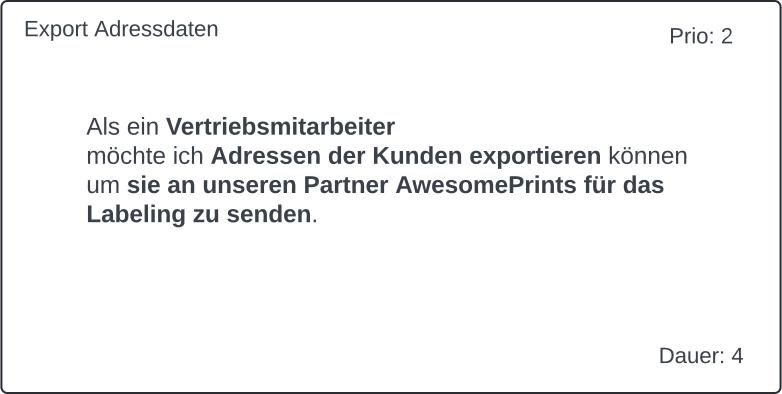
\includegraphics[scale=0.4]{chapters/Anhang/CheatSheets/img/StoryCard}
    \caption{Beispiel für eine \textbf{User Story} in Form einer \textbf{Story Card} mit Titel und Beschreibung sowie Angabe der Priorität und geschätzten Dauer zur Umsetzung. (Quelle: eigene)}
    \label{fig:storycard}
\end{figure}